% !TEX program = pdflatex
% !TEX encoding = UTF-8 Unicode

% General TODOs
% [ ] Remove `dedicatoria.tex`, we already have `agradecimientos.tex`
% [ ] Remove the use of apendixes, we are not using them yet

% Sergio Quijano Rey
% Doble Grado Ingenieria Informatica y Matematicas, UGR
% A partir de la plantilla dada en la página del grado de matemáticas de la UGR
% Dicha plantilla se puede descargar desde https://grados.ugr.es/informatica/pages/infoacademica/tfg/plantillas/plantilla_tfg_latex/!

% Usamos un documentclass propio del paquete KOMA-script
\documentclass{scrbook}

% Opciones del paquete KOMA-script
% Son las dadas por defecto en la plantilla, que sigue las directrices del TFG
\KOMAoptions{%
  fontsize=10pt,        % Tamaño de fuente
  paper=a4,             % Tamaño del papel
  headings=normal,      % Tamaño de letra para los títulos: small, normal, big
  % parskip=half,         % Espacio entre párrafos: full (una línea) o half (media línea)
  headsepline=false,    % Una linea separa la cabecera del texto
  cleardoublepage=empty,% No imprime cabecera ni pie en páginas en blanco
  chapterprefix=false,  % No antepone el texto "capítulo" antes del número
  appendixprefix=false,	% No antepone el texto "Apéndice" antes de la letra
  listof=totoc,		    	% Añade a la tabla de contenidos la lista de tablas y figuras
  index=totoc,			    % Añade a la talba de contenidos una entrada para el índice
  bibliography=totoc,	  % Añade a la tabla de contenidos una entrada para bibliografía
  BCOR=5mm,           % Reserva margen interior para la encuadernación.
                        % El valor dependerá el tipo de encuadernado y del grosor del libro.
  DIV=10,             % Cálcula el diseño de página según ciertos
                        % parámetros. Al aumentar el número aumentamos el ancho de texto y disminuimos el ancho del margen. Una opción de 14 producirá márgenes estrechos y texto ancho.
}

% TODO -- mirar esto cuando vaya a imprimir el TFG
% INFORMACIÓN PARA LA VERSIÓN IMPRESA
% Si el documento ha de ser impreso en papel de tamaño a4 pero el tamaño del documento (elegido en \KOMAoptions con la ocpión paper) no es a4 descomentar la línea que carga el paquete `crop` más abajo. El paquete crop se encargará de centrar el documento en un a4 e imprimir unas guías de corte. El procedimiento completo para imprenta sería el siguiente:
% 0. Determinar, según el tipo de encuadernación del documento, el ancho reservado para el proceso de encuadernación (preguntar en la imprenta), es decir, la anchura del área del papel que se pierde durante el proceso de encuadernación. Fijar la varibale BCOR de \KOMAoptions a dicho valor.
% 1. Descomentar la siguiente línea e imprimir una única página con las guías de corte
% 2. Cambiar la opción `cross` por `cam` (o `off`) en el paquete crop y volver a compilar. Imprimir el documento (las guías de corte impresas no inferfieren con el texto).
% 3. Usar la página con las guías impresas en el punto 1 para cortar todas las páginas.

% \usepackage[a4, odd, center, pdflatex, cross]{crop} % Permite imprimir el documento en un a4 (si el tamaño es más pequeño) mostrando unas guías de corte. Útil para imprenta.

% ---------------------------------------------------------------------
%	PAQUETES
% ---------------------------------------------------------------------

% CODIFICACIÓN E IDIOMA
% ---------------------------------------------------------------------
\usepackage[utf8]{inputenc} 			    % Codificación de caracteres

% Selección del idioma: cargamos por defecto inglés y español (aunque este último es el idioma por defecto para el documento). Cuando queramos cambiar de idioma escribiremos:
% \selectlanguage{english} o \selectlanguage{spanish}

\usepackage[english, spanish, es-nodecimaldot, es-noindentfirst, es-tabla]{babel}

% Opciones cargadas para el paquete babel:
  % es-nodecimaldot: No cambia el punto decimal por una coma en modo matemático.
  % es-noindentfirst: No sangra los párrafos tras los títulos.
  % es-tabla: cambia el título del entorno `table` de "Cuadro" a "Tabla"

% Otras opciones del paquete spanish-babel:
  \unaccentedoperators % Desactiva los acentos en los operadores matemáticso (p.e. \lim, \max, ...). Eliminar esta opción si queremos que vayan acentuados

% MATEMÁTICAS
% ---------------------------------------------------------------------
\usepackage{amsmath, amsthm, amssymb} % Paquetes matemáticas
\usepackage{mathtools}                % Añade mejoras a amsmath
\mathtoolsset{showonlyrefs=true}      % sólo se numeran las ecuaciones que se usan
\usepackage[mathscr]{eucal} 					% Proporciona el comando \mathscr para
                                      % fuentes de tipo manuscrito en modo matemático sin sobreescribir el comando \mathcal

% TIPOGRAFÍA
% ---------------------------------------------------------------------
% El paquete microtype mejora la tipografía del documento.
\usepackage[activate={true,nocompatibility},final,tracking=true,kerning=true,spacing=true,factor=1100,stretch=10,shrink=10]{microtype}

% TODO -- para el codigo creo que es mejor fuente Cascadia Code (preferencia personal)
% Las tipografías elegidas para el documento, siguiendo la guía de estilo de la UGR,
% son las siguientes
% Normal font: 			URW Palladio typeface.
% Sans-serif font: 	Gill Sans
% Monospace font: 	Inconsolata
\usepackage[T1]{fontenc}
\usepackage[sc, osf]{mathpazo} \linespread{1.05}
\usepackage[scaled=.95,type1]{cabin} % sans serif in style of Gill Sans
% Si el paquete cabin da error usar el siguiente comando en su lugar
% \renewcommand{\sfdefault}{iwona}
\usepackage{inconsolata}


% Selecciona el tipo de fuente para los títulos (capítulo, sección, subsección) del documento.
\setkomafont{disposition}{\sffamily\bfseries}

% Cambia el ancho de la cita. Al inicio de un capítulo podemos usar el comando \dictum[autor]{cita} para añadir una cita famosa de un autor.
\renewcommand{\dictumwidth}{0.45\textwidth}

\recalctypearea % Necesario tras definir la tipografía a usar.

\usepackage{setspace}
% TABLAS, GRÁFICOS Y LISTADOS DE CÓDIGO
% ---------------------------------------------------------------------
\usepackage{booktabs}
% \renewcommand{\arraystretch}{1.5} % Aumenta el espacio vertical entre las filas de un entorno tabular

\usepackage{xcolor, graphicx}
% Carpeta donde buscar los archivos de imagen por defecto
\graphicspath{{img/}}

% IMAGEN DE LA PORTADA
% Existen varias opciones para la imagen de fondo de la portada del TFG. Todas ellas tienen en logotipo de la universidad de Granada en la cabecera. Las opciones son las siguientes:
% 1. portada-ugr y portada-ugr-color: diseño con marca de agua basada en el logo de la UGR (en escala de grises y color).
% 2. portada-ugr-sencilla y portada-ugr-sencilla-color: portada únicamente con el logotipo de la UGR en la cabecera.
\usepackage{eso-pic}
\newcommand\BackgroundPic{%
	\put(0,0){%
		\parbox[b][\paperheight]{\paperwidth}{%
			\vfill
			\centering
      % Indicar la imagen de fondo en el siguiente comando
			
\includegraphics[width=\paperwidth,height=\paperheight,%
			keepaspectratio]{portada-ugr-sencilla}%
			\vfill
}}}

% \usepackage{listings} % Para la inclusión de trozos de código

% CABECERAS
% ---------------------------------------------------------------------
% Si queremos modificar las cabeceras del documento podemos usar el paquete
% `scrlayer-scrpage` de KOMA-Script. Consultar la documentación al respecto.
% \usepackage[automark]{scrlayer-scrpage}

% VARIOS
% ---------------------------------------------------------------------

%\usepackage{showkeys}	% Muestra las etiquetas del documento. Útil para revisar las referencias cruzadas.

% ÍNDICE
% Para generar el índice hay que compilar el documento con MakeIndex. Generalmente los editores se encargan de ello automáticamente.
% ----------------------------------------------------------------------
% \index{} para añadir un elemento
% \index{main!sub} para añadir un elementos "sub" bajo la categoría "main".
% \index{termino|textbf} para dar formato al número de página (negrita).
% \index{termino|see{termino relacionado}} para crear una referencia cruzada

% Ejemplo: \index{espacio homogéneo}, \index{superficie!mínima}, \index{esfera|see{espacio homogéneo}}

% Activar los siguientes comandos para generar el índice terminológico. Ver también comandos al final de este documento para incluir dicho índice en el pdf final.
% \usepackage{makeidx}
% \makeindex

% Para revisar las entradas al índice conforme las incluimos en el documento es útil el siguiente paquete. Conviene observar que mientras esté cargado no se generará el índice.
%\usepackage{showidx} % Muestra en el margen del documento las entradas añadidas al índice. Útil para revisar el documento. Si está activo el índice no se genera

% Mis librerias cargadas
%====================================================================================================
\usepackage{listings}

% ---------------------------------------------------------------------
% COMANDOS Y ENTORNOS
% ---------------------------------------------------------------------
% Cargamos un archivo externo donde hemos incluido todos los comandos
% propios que vamos a usar en el documento.
% == Comandos de la plantilla ==
% ==============================================================================

\newcommand{\N}{\mathbb{N}}     % Naturales
\newcommand{\R}{\mathbb{R}}     % Reales
\newcommand{\Z}{\mathbb{Z}}     % Enteros
\newcommand{\Q}{\mathbb{Q}}     % Racionales
\newcommand{\C}{\mathbb{C}}     % Complejos

% TEOREMAS Y ENTORNOS ASOCIADOS

% \newtheorem{theorem}{Theorem}[chapter]:
\newtheorem*{teorema*}{Teorema}
\newtheorem{teorema}{Teorema}[chapter]
\newtheorem{proposicion}{Proposición}[chapter]
\newtheorem{lema}{Lema}[chapter]
\newtheorem{corolario}{Corolario}[chapter]

\theoremstyle{definition}
\newtheorem{definicion}{Definición}[chapter]
\newtheorem{ejemplo}{Ejemplo}[chapter]

\theoremstyle{remark}
\newtheorem{observacion}{Observación}[chapter]

% == Mis comandos propios ==
% ==============================================================================

% Comando que uso para expresar el conjunto {1, ..., param_1}
\newcommand{\deltaset}[1]{\Delta_{#1}}

% Comando que uso para expresar el conjunto {param_1, ..., param_2}
\newcommand{\doubledeltaset}[2]{\Delta_{#1}^{#2}}


% Espacio de matrices pxq
\newcommand{\espaciomatrices}[2]{\mathbb{M}_{#1 \times #2}}

% Espacio de tensores de orden N, #1 y de dimension M, #2 en cada modo
\newcommand{\espaciotensores}[2]{\mathcal{T}_{#1, #2}}

% Un mejor simbolo para QED
% Hago el renew para que \begin{proof} \end{proof} muestre este simbolo como a mi me gusta
\newcommand{\customqed}{\hfill\blacksquare}
\renewcommand{\qedsymbol}{$\customqed$}

% Elementos con explicaciones encima:

% Para poner cualquier cosa encima de otra dada
\newcommand{\encima}[2]{\ensuremath{\stackrel{#2}{#1}}}

% Igualdades
\newcommand{\eqtext}[1]{\ensuremath{\stackrel{\text{#1}}{=}}}
\newcommand{\eqmath}[1]{\ensuremath{\stackrel{#1}{=}}}

% Implicaciones
\newcommand{\impliestext}[1]{\ensuremath{\stackrel{\text{#1}}{\implies}}}

% Comando para indicar algun tipo de isomorfismo
\newcommand{\isomorfismo}[1]{\underset{#1}{\cong}}

% Expresiones logicas mas sencillas
\newcommand{\then}{\implies}
\newcommand{\iif}{\Longleftrightarrow}

% Algunos vectores que usamos bastante
\newcommand{\vectordd}[2]{\begin{pmatrix} #1 \\ #2 \end{pmatrix}}
\newcommand{\vectorn}[3]{\begin{pmatrix} #1 \\ #2 \\ \vdots \\ #3 \end{pmatrix}}

% Dos espacios
\newcommand{\dspace}{\ \ }

% Espacio de tensores de orden N (#1) y dimension M (#2) en cada modo
% TODO -- ahora estoy usando \espaciotensores que es mejor notacion
\DeclareMathOperator*{\MediumOtimes}{\text{\raisebox{0.25ex}{\scalebox{0.8}{$\bigotimes$}}}}
\newcommand{\esptensores}[2]{\overset{#1} \MediumOtimes \R^{#2}}

% (N)otacion para los (v)ectores => (nv)
% En el paper usan negrita, pero yo quiero usar una flechita encima
% Con este comand, si luego quiero cambiar la notación para los vectores (ie. volver
% a usar la notacion del paper) el cambio es sencillo
%
% NOTE: para poder usarse tiene que estar en un bloque de matematicas, por ejemplo:
% `$\nv{x}$`
\newcommand{\nv}[1]{\overrightarrow{#1}}

\newcommand{\entrecomillado}[1]{\textit{``#1''}}

% Forma mas comoda para escribir el producto escalar
\newcommand{\innerproduct}[2]{\langle #1 \; | \; #2 \rangle}

% Para añadir comentarios debajo o encima de elementos de una formula
\newcommand{\comentardebajo}[2]{\underbrace{#1}_\textrm{#2}}
\newcommand{\comentarencima}[2]{\overbrace{#1}^\textrm{#2}}

% Comando para evitar que las captions de las subfiguras colisionen entre si
\newcommand{\ajustarsubcaptions}{\captionsetup[subfigure]{width=0.9\textwidth,position=b}}

% Comando para escribir conjuntos matematicos
\newcommand{\conjunto}[1]{\{ #1 \}}

% Para escribir union e interesccion
\newcommand{\interseccion}{\bigcap}
\newcommand{\union}{\bigcup}

% Para hacer `\to` pero de forma larga, como con \longmapsto
\newcommand{\longto}{\longrightarrow}

% Para hacer el conjunto de combinaciones lineales `span`
% Cuidado porque hay un comando de latex que ya se llama span
\newcommand{\spansetlong}[2]{\text{span}_{#1} \conjunto{#2}}
\newcommand{\spanset}[1]{\spansetlong{\mathbb{R}}{#1}}

% El paquete `cleveref` usa los nombres de secciones en ingles, los necesito
% en español
\Crefname{section}{Sección}{Sección}
\crefname{section}{Sección}{Sección}
\Crefname{chapter}{Capítulo}{Sección}
\crefname{chapter}{Capítulo}{Capítulo}

% Comandos para referenciar
\newcommand{\imgref}[1]{\Cref{#1}}
\newcommand{\sectionref}[1]{\Cref{#1}}
\newcommand{\coderef}[1]{\Cref{#1}}
\newcommand{\tableref}[1]{\Cref{#1}}
\newcommand{\propref}[1]{\Cref{#1}}

% Deberiamos evitar el uso de este comando generico
\newcommand{\customref}[1]{\Cref{#1}}


% --------------------------------------------------------------------
% INFORMACIÓN DEL TFG Y EL AUTOR
% --------------------------------------------------------------------
\usepackage{xspace} % Para problemas de espaciado al definir comandos

% TODO -- hay que poner un titulo al trabajo
% TODO -- hay que poner informacion de los tutores
\newcommand{\miTitulo}{Título del trabajo\xspace}
\newcommand{\miNombre}{Sergio Quijano Rey\xspace}
\newcommand{\miGrado}{Doble Grado en Ingeniería Informática y Matemáticas}
\newcommand{\miFacultad}{Facultad de Ciencias, Escuela Superior Ingeniería Informática y Telecomunicaciones}
\newcommand{\miUniversidad}{Universidad de Granada}
% Añadir tantos tutores como sea necesario separando cada uno de ellos
% mediante el comando `\medskip` y una línea en blanco
\newcommand{\miTutor}{
  Nombre del tutor 1 \\ \emph{Departamento del tutor 1}

  % Añadir tantos tutores como sea necesario.

  \medskip
  Nombre del tutor 2 \\ \emph{Departamento del tutor 2}
}
\newcommand{\miCurso}{2020-2021\xspace}

% HYPERREFERENCES
% --------------------------------------------------------------------
\usepackage{xurl}
\usepackage{hyperref}
% Opciones para el paquete hyperref
%----------------------------------

\hypersetup{%
  % hidelinks,            % Enlaces sin color ni borde. El borde no se imprime
  linkbordercolor=0.8 0 0,
  citebordercolor=0 0.8 0,
  citebordercolor=0 0.8 0,
  colorlinks = true,            % Color en texto de los enlaces. Comentar esta línea o cambiar `true` por `false` para imprimir el documento.
  linkcolor = [rgb]{0.5, 0, 0}, % Color de los enlaces internos
  urlcolor = [rgb]{0, 0, 0.5},  % Color de los hipervínculos
  citecolor = [rgb]{0, 0.5, 0}, % Color de las referencias bibliográficas
	pdftitle={\miTitulo},%
	pdfauthor={\textcopyright\ \miNombre, \miFacultad, \miUniversidad},%
  pdfsubject={Trabajo de fin de Grado},%
	pdfkeywords={},%
	pdfcreator={pdfLaTeX},%
}

% Redefinición del estilo para mostrar las referencias cruzadas en la bibliografía.
% \renewcommand*{\backref}[1]{}
% \renewcommand{\backrefsep}{, }
% \renewcommand{\backreftwosep}{ y }
% \renewcommand{\backreflastsep}{ y }
% \renewcommand*{\backrefalt}[4]{{\footnotesize [%
%     \ifcase #1 No citado%
%     \or Citado en pág.~#2%
%     \else Citado en págs. #2%
%     \fi%
% ]}}

% Etiquetas en español para el comando \autoref
\def\chapterautorefname{Capítulo}
\def\appendixautorefname{Apéndice}
\def\sectionautorefname{Sección}
\def\subsectionautorefname{Subsección}
\def\figureautorefname{Fig.}
\def\tableautorefname{Tabla}

\def\teoremaautorefname{Teorema}
\def\proposicionautorefname{Proposición}
\def\lemaautorefname{Lema}
\def\corolarioautorefname{Corolario}
\def\definicionautorefname{Def.}
\def\observacionautorefname{Observación}
\def\ejemploautorefname{E.j.}

% Pone automáticamente un parántesis para las ecuaciones
\def\equationautorefname~#1\null{(#1)\null}


\begin{document}

% --------------------------------------------------------------------
% FRONTMATTER
% -------------------------------------------------------------------
\frontmatter % Desactiva la numeración de capítulos y usa numeración romana para las páginas

% \pagestyle{plain} % No imprime cabeceras

% !TeX root = ../libro.tex
% !TeX encoding = utf8

%*******************************************************
% Titlepage
%*******************************************************
\begin{titlepage}
  \AddToShipoutPicture*{\BackgroundPic}
  \phantomsection
  \pdfbookmark[1]{Título}{title}

  % Para que el título esté centrado en la página.
  % Los valores numéricos deberán elegirse de acuerdo con el diseño de
  % página (sobre todo si se cambia la opción BCOR o DIV).
  \begin{addmargin}[2.575cm]{0cm}
  \begin{flushleft}
    \Large
    \hfill\vfil

    \large{\textsf{\miFacultad}}
    \vfill

    {\large\textsc\miGrado} \vfill


    {\large\textsc{trabajo de fin de grado}}

    \begin{flushleft}
      \Huge
      \setstretch{0.8}
      \miTitulo
    \end{flushleft}

    \vfill\vfill\vfill\vfill

    \textsf{\normalsize{Presentado por:}}\\
    {\normalsize\textrm{\miNombre}}
    \bigskip

    \textsf{\normalsize{Tutores:}}\\
    {\normalsize\rmfamily\miTutor}

    \bigskip
    \textsf{\normalsize{Curso académico \miCurso}}
  \end{flushleft}
  \end{addmargin}

\end{titlepage}
\cleardoublepage
\endinput

% !TeX root = ../libro.tex
% !TeX encoding = utf8

%*******************************************************
% Little Dirty Titlepage
%*******************************************************

\thispagestyle{empty}

\begin{center}
  \large  

  \vspace*{\stretch{1}}

  \begingroup
  \huge{\miTitulo} \\ \bigskip
  \endgroup

  \textrm{\miNombre}

  \vspace{\stretch{5}}

\end{center}  

\newpage
\thispagestyle{empty}

\hfill

\vfill

\miNombre \textit{\miTitulo}.

Trabajo de fin de Grado. Curso académico \miCurso.
\bigskip

\begin{minipage}[t]{0.25\textwidth}
  \flushleft
  \textbf{Responsable de tutorización}
\end{minipage}
\begin{minipage}[t]{0.45\textwidth}
  \flushleft
  \miTutor
\end{minipage}
\begin{minipage}[t]{0.30\textwidth}
  \flushright
  \miGrado
  \medskip

  \miFacultad
  \medskip

  \miUniversidad
\end{minipage}

\newpage
\endinput

% !TeX root = ../libro.tex
% !TeX encoding = utf8
%
%*******************************************************
% Declaración de originalidad
%*******************************************************

\thispagestyle{empty}

\hfill\vfill

\textsc{Declaración de originalidad}\\\bigskip

D./Dña. \miNombre \\\medskip

Declaro explícitamente que el trabajo presentado como Trabajo de Fin de Grado (TFG), correspondiente al curso académico \miCurso, es original, entendida esta, en el sentido de que no ha utilizado para la elaboración del trabajo fuentes sin citarlas debidamente.
\medskip

En Granada a \today 
\begin{flushleft} 
Fdo: \miNombre 

\end{flushleft}

\vfill

\cleardoublepage
\endinput

% !TeX root = ../libro.tex
% !TeX encoding = utf8

%*******************************************************
% Dedication
%*******************************************************
\thispagestyle{empty}
\phantomsection 
\pdfbookmark[1]{Dedicatoria}{Dedicatoria}

\hfill
\vfill

\begin{flushright}
\itshape
Dedicatoria (opcional) \\
Ver archivo \texttt{preliminares/dedicatoria.tex}
\end{flushright}

\vfill

\cleardoublepage
\endinput
                % Opcional
% !TeX root = ../libro.tex
% !TeX encoding = utf8

%*******************************************************
% Table of Contents
%*******************************************************
\phantomsection
\pdfbookmark[0]{\contentsname}{toc}

\setcounter{tocdepth}{2} % <-- 2 includes up to subsections in the ToC
\setcounter{secnumdepth}{3} % <-- 3 numbers up to subsubsections

% \manualmark
% \markboth{\textsc{\contentsname}}{\textsc{\contentsname}}
\tableofcontents

% Sergio: modifico este archivo para que se incluyan en el indice las figuras, tablas y codigos


%*******************************************************
% List of Figures and of the Tables
%*******************************************************

    % *******************************************************
    %  List of Figures
    % *******************************************************
    % \phantomsection
    \listoffigures

    %*******************************************************
    % List of Tables
    %*******************************************************
    % \phantomsection
    \listoftables

    %*******************************************************
    % List of Listings
    % The package \usepackage{listings} is needed
    %*******************************************************
      % \phantomsection
    \renewcommand{\lstlistlistingname}{Listados de código}
    \lstlistoflistings

\cleardoublepage

% !TeX root = ../libro.tex
% !TeX encoding = utf8

%*******************************************************
% Agradecimientos
%*******************************************************

\chapter{Agradecimientos}

Agradecimientos del libro (opcional, ver archivo \texttt{preliminares/agradecimiento.tex}).

\cleardoublepage
\endinput
            % Opcional

% \pagestyle{scrheadings} % A partir de ahora sí imprime cabeceras

% !TeX root = ../libro.tex
% !TeX encoding = utf8
%
%*******************************************************
% Summary
%*******************************************************

% TODO -- lo tengo que escribir, porque es una parte obligatoria

\selectlanguage{english}
\chapter{Summary}

\todo{Escribirlo cuando la parte de informática se estabilice algo}

An english summary of the project (around 800 and 1500 words are recommended).

File: \texttt{preliminares/summary.tex}


% Al finalizar el resumen en inglés, volvemos a seleccionar el idioma español para el documento
\selectlanguage{spanish}
\endinput

% !TeX root = ../libro.tex
% !TeX encoding = utf8
%
%*******************************************************
% Introducción
%*******************************************************

% \manualmark

% \markboth{\textsc{Introducción}}{\textsc{Introducción}}

\chapter{Resumen}

% 1. Objetivos
% 1. Papers principales con los que trabajamos
% 1. Objetivos alcanzados y objetivos no alcanzados
% 1. Estado del arte

\textbf{Palabras clave}: Análisis Tensorial, Descomposición Tensorial \textit{CP}, Descomposición Tensorial \textit{HT}, Aprendizaje Automático, Aprendizaje Profundo, Visión por Computador, Redes Convolucionales, Reconocimiento Facial Invariante a la Edad, \textit{Triplet Loss}

El presente Trabajo de Fin de Grado tiene dos \textbf{objetivos principales}. El primero de ellos consiste en realizar una modelización de las redes neuronales convolucionales, profundas y no profundas, y estudiar la propiedad conocida comúnmente como \textit{depth efficiency}. El segundo objetivo consiste en resolver una tarea de reconocimiento facial invariante a cambios en la edad. Además, estudiaremos ciertas variantes sobre la función de pérdida \textit{Triplet Loss}, buscando resolver algunos problemas asociados al uso de esta técnica. Dichas variantes suponen un gran esfuerzo de implementación, por lo tanto, buscamos aplicar patrones de diseño para que la arquitectura resultante sea fácil de modificar y extender.

El uso de técnicas de aprendizaje automático basado en redes neuronales profundas ha crecido enormemente en los últimos años. Su buen rendimiento en ciertas tareas específicas ha sido demostrado de forma contundente. Sin embargo, este buen rendimiento \textbf{se justifica únicamente sobre la evidencia experimental}. No se realizado un estudio profundo y fructífero sobre los motivos teóricos que respaldan los resultados experimentales. Los trabajos que realizan un estudio para respaldar la línea experimental suelen trabajar con modelizaciones matemáticas alejadas de los modelos comunes del \textit{deep learning}, y los resultados suelen tratar sobre casos concretos en los que las redes profundas son claramente superiores a las redes no profundas o \textit{shallow}. La publicación con la que trabajamos principalmente es \cite{matematicas:principal}.

Nuestro trabajo en esta línea es novedoso por dos motivos principales: la \textbf{modelización matemáticas de las redes neuronales es muy cercana a la realidad}, y el resultado sobre \textbf{\textit{depth efficiency} da información concreta sobre la cantidad de escenarios} en los que ocurre esta \textit{depth efficiency}.

Expresaremos las funciones de puntuación que la red busca aprender en base a un tensor de coeficientes sobre una base de funciones linealmente independientes y totales. A partir de aquí, la modelización se basa en dos conocidas descomposiciones tensoriales, la descomposición \textit{CANDECOMP/PARAFAC} o \textit{CP} y la descomposición jerárquica \textit{Tucker} o \textit{HT}. Estas \textbf{modelizaciones tienen en cuenta las propiedades fundamentales de las redes convolucionales}: localidad de la convolución, compartición de coeficientes y operadores de \textit{pooling}.

Demostraremos \textbf{dos resultados centrales}. El primero nos muestra que, en el sentido de la medida de Lebesgue, casi todos los modelos no profundos necesitan un número exponencial de parámetros para implementar un modelo profundo. El segundo resultado añade que, de hecho, casi todos los modelos profundos no pueden ni siquiera ser aproximados por un modelo no profundo con menos de un número exponencial de parámetros.

En esta línea, \textbf{los objetivos de este estudio han sido alcanzados}. Hemos presentado una modelización matemática muy cercana a la realidad, y hemos demostrado dos resultados que nos dan información exacta sobre en qué escenarios son superiores las redes profundas frente a las redes no profundas, y cómo de frecuente sucede esto.

Por otro lado, hemos \textbf{intentado resolver una tarea de reconocimiento facial invariante a la edad, o \textit{AIFR}}. Esta tarea resulta muy interesante en el ambiente de la \textbf{informática forense}, por todas las aplicaciones prácticas que tiene obtener un modelo capaz de identificar a un individuo en distintas imágenes independientemente de la edad con la que aparezca en dichas imágenes. Buscamos aplicar las técnicas introducidas en la publicación \cite{informatica:principal} en la tarea de \textit{AIFR}, enfoque que según nuestro conocimiento nunca se había aplicado a esta tarea.

Dicha tarea presenta una complejidad elevada. Además de los retos que supone una tarea de visión por computador usual, debemos añadir todos los \textbf{retos asociados a cómo el envejecimiento afecta las características faciales} con las que trabajamos.

Para resolver el problema planteado, realizamos un estudio del estado del arte, que nos indica las principales líneas de trabajo que más éxito han tenido. Estos trabajos utilizan principalmente redes generativas adversarias para descomponer los datos de entrada en dos características incorreladas: edad e identidad. Algunos trabajos utilizando modelos basados en atención para aprender a resolver esta tarea. Este enfoque usa técnicas y modelos avanzados, que quedan fuera del alcance del presente trabajo.

Realizamos un estudio de los conjuntos de datos disponibles. Estos son escasos y en ocasiones de una calidad pobre. Estudiamos el tamaño de los conjuntos de datos, las distribuciones del número de imágenes por individuo (fundamental para aplicar nuestras técnicas), la distribución de edad de los individuos y la distribución del rango de edad de los individuos. En base a este estudio tomamos una decisión informada de qué conjuntos usar y qué protocolo experimental aplicar. Siguiendo la línea más común en el estado del arte, entrenamos sobre un conjunto de datos grande, \textit{CACD}, y validamos sobre el conjunto \textit{FG-Net}, que presenta un gran reto por su gran variedad en edades y rangos.

Desarrollamos una amplia base de código para poder aplicar las técnicas estudiadas. Realizamos una optimización de la base de código guíada por los datos tomados durante varios \textit{profiles}, debido a necesidades de rendimiento. Por los malos resultados obtenidos, aplicamos una amplia \textit{suite} de \textit{tests} para validar que los malos resultados no estén provocados por fallos en la implementación.

Realizamos una \textbf{experimentación y estudio de los resultados}. Eston son pésimos, muy lejos de ser competitivos con el estado del arte y, todavía peor, muy lejanos de ser aplicables en un escenario práctico. El estado del arte obtiene valores para \textit{Rank@1 Accuracy} superiores al 90\%. Nuestro modelo no llega al 0.1\%. Además, al no existir literatura concreta sobre el uso de estas técnicas sobre un problema de \textit{AIFR}, debemos justificar los pésimos resultados en base al presente trabajo.

Por lo tanto, \textbf{se ha cumplido el objetivo de desarrollar una base de código bien diseñada}, con la que sea cómodo trabajar y experimentar. Sin embargo, los \textbf{resultados experimentales son muy malos y quedan muy lejos de los objetivos propuestos} inicialmente.

\endinput


% --------------------------------------------------------------------
% MAINMATTER
% --------------------------------------------------------------------
\mainmatter % activa la numeración de capítulos, resetea la numeración de las páginas y usa números arábigos

\setpartpreamble[c][0.75\linewidth]{%
	\bigskip % Deja un espacio vertical en la parte superior
  Si el trabajo se divide en diferentes partes es posible incluir al inicio de cada una de ellas un breve resumen que indique el contenido de la misma. Esto es opcional.
}
\part{Primera parte}

\chapter{Introducción}\label{ch:introduccion}

El objetivo de este trabajo, desde la perspectiva de las matemáticas, es \textbf{analizar las redes neuronales profundas basadas en convoluciones y explicar por qué en ciertos escenarios éstas funcionan mejor que las redes neuronales no profundas}, a las que llamaremos redes someras. En este escenario ocurre que para replicar redes profundas con un número polinomial de coeficientes, necesitamos que las redes someras tengan un número de coeficientes superior al polinomial, concretamente, exponencial. En este caso hablamos de \textbf{eficiencia en profundidad} o \textbf{\entrecomillado{depth efficiency}}.
\todo{Poner aquí una referencia a otra parte del paper sobre esto de tamaño exponencial}

La eficiencia en profundidad es muy conocida en la práctica, pero pocos son los trabajos que han tratado de justificar matemáticamente por qué ocurre este fenómeno. Además, como se comenta en \cite{matematicas:principal}, \textbf{en la mayoría de trabajos de este tipo, no se han tenido en cuenta propiedades fundamentales de las redes profundas ni de las redes convolucionales} \cite{matematicas:paper_depth_malo_01} \cite{matematicas:paper_depth_malo_02} \cite{matematicas:paper_depth_malo_03}. Por otro lado, suelen ser trabajos en los que \textbf{se muestran ejemplos concretos} de funciones implementables (de forma eficiente) con redes profundas pero no con redes someras, sin dar \textbf{ningún tipo de información sobre con qué frecuencia ocurre esto}. En base a esto, las \textbf{principales fortalezas de este trabajo respecto a otros} es que consideramos:
\todo{Comentarios de JMeri: este tipo de afirmaciones pueden llevar a preguntas del tribunal. Preparar bien las posibles respuestas}
\todo{Quizás yo añadir comentarios sobre esta afirmación para que se responda automáticamente al leer esto}

\begin{itemize}
	\item La diferencia jerárquica entre ambos tipos de redes.
	\item Propiedades fundamentales de las redes convolucionales: compartición de los coeficientes en las convoluciones, localidad de la operación de convolución y uso de la operación de \textit{pooling}.
	\item Un estudio de lo frecuente que es tener funciones que sean implementables (de forma eficiente) por redes profundas pero no por redes someras.
\end{itemize}
\todo{Desarrollar más qué significan estas propiedades. En la introducción del paper se explica esto más o menos}

\section{Objetivos}

Los principales \textbf{objetivos} del presente trabajo son los siguientes. Como punto de partida, modelar matemáticamente la tarea de aprendizaje representando los datos de entrada, la tarea a resolver y el espacio de hipótesis en el que buscaremos la mejor solución. Posteriormente, modelar los dos tipos de redes neuronales (profundas y someras) a través de dos tipos de descomposiciones tensoriales. La descomposición \textit{CP}, que equivale al uso de redes someras y que desarrollamos en la \sectionref{subs:descomposcion_cp}. Y la descomposición \textit{HT}, que equivale al uso de redes profundas y que introducimos en la \sectionref{subs:descomposicion_ht}. Finalmente, demostrar dos resultados centrales que pondrán de manifiesto la superioridad de las redes profundas, en lo que se conoce como eficiencia en profundidad, a través de las ya mencionadas descomposiciones tensoriales.

El primer resultado central, el \propref{teorema:teorema_principal_especificacion}, dice que si tenemos un modelo profundo con un número polinomial de coeficientes, el modelo somero necesitará al menos un número exponencial de coeficientes para poder implementar el mismo modelo. Esto ocurre casi por doquier respecto al espacio de los coeficientes que determinan el modelo profundo. El segundo resultado central, el \propref{corolario:corolario_principal_concreto}, indica que no es que un modelo somero no pueda realizar el modelo profundo con menos de un número exponencial de parámetros, sino que no es capaz ni de aproximar al modelo profundo con menos de un número exponencial de parámetros. De nuevo, esto ocurre casi por doquier respecto al espacio de los coeficientes que determinan el modelo profundo.

Nos basaremos principalmente en el trabajo \cite{matematicas:principal}. Algunas de las herramientas que usaremos serán la teoría básica sobre tensores, las descomposiciones tensoriales \textit{CP} y \textit{HT}, la matrización de tensores, algunos resultados conocidos sobre la medida de Lebesgue y finalmente el álgebra de matrices básica.

\section{Estructura del trabajo}

La estructura del trabajo será la siguiente. En primer lugar, en el \sectionref{ch:matematicas_fundamentales} introduciremos las herramientas básicas sobre las que fundamentaremos nuestro trabajo. En concreto, introduciremos el concepto de producto tensorial. En segundo lugar, en el \sectionref{ch:tarea_aprendizaje} indicaremos cómo representamos matemáticamente la tarea de aprendizaje. Para ello, modelizaremos un espacio de hipótesis general, para lo cual justificaremos la elección de ciertas funciones de puntuación, que serán clave en el desarrollo del trabajo, y la elección de determinadas funciones de representación. En la \sectionref{subs:capa_de_representacion} daremos un primer paso común en la modelización de ambas arquitecturas de aprendizaje automático, presentando la primera capa de ambos modelos. En tercer lugar, en el \sectionref{ch:modelizacion} desarrollaremos las dos modelizaciones (somera y profunda) a partir de dos descomposiciones tensoriales (\textit{CP} y \textit{HT}, respectivamente). Veremos en ambos casos cómo las modelizaciones realizadas se corresponden con arquitecturas usadas en la práctica del aprendizaje automático. Compararemos el número de parámetros que definen cada modelo, pues será fundamental en nuestros resultados teóricos. En cuarto lugar, en el \sectionref{chapter:teoremas_y_demostraciones} introduciremos los dos resultados principales, veremos y demostraremos algunos resultados previos necesarios para las demostraciones y probaremos el teorema y corolario principal. En quinto y último lugar, en el \sectionref{chapter:conclusiones_trabajo_futuro} comentaremos los resultados obtenidos a partir del presente trabajo e introduciremos posibles líneas de estudio en base a nuestros resultados.

% Añadir tantos capítulos como sea necesario

\cleardoublepage\part{Segunda parte}
\chapter{Fundamentos teóricos} \label{ich:fundamentos_teoricos}

En esta sección introduciremos algunos \textbf{conceptos teóricos} sobre los que se basará nuestro trabajo, y por tanto, conviene conocer para entender este trabajo.

\section{\textit{Embeddings}} \label{isec:embeddings}

Nuestro trabajo busca desarrollar un modelo de aprendizaje automático que aprenda un \textit{embedding}. Un \textit{embedding} no es más que un mapeo desde un cierto espacio $X$ de datos de entrada (en nuestro caso, podemos considerar $X$ como el espacio de imágenes en las que aparecen caras) a un espacio vectorial $\R^N$. En la mayoría de casos, la dimensión del espacio de llegada $N$ es menor que la dimensión del espacio $X$.

Más formalmente, buscamos aprender una función

\begin{equation}
\begin{split}
    f_{\theta}: X & \to \R^N \\
    x & \mapsto f_{\theta}(x)
\end{split}
\end{equation}

que tomamos de una familia paramétrica de funciones $\{f_{\theta}: \theta \in \Theta \}$. En el caso de nuestro problema, podemos pensar en la familia de los modelos profundos de redes convolucionales ($\theta$ estaría por tanto compuesto por todos los coeficientes que determinan dicho modelo convolucional, luego podríamos pensar en $\Theta \subseteq \R^M$ donde $M$ es el número de coeficientes del modelo).

El criterio para escoger una función u otra de mapeo es que este deberá ser \textbf{semántico}. En el espacio de llegada $\R^N$ tenemos una métrica:

\begin{equation}
\begin{split}
    D: X \times X & \to [0, \infty) \\
    x, y & \mapsto D(x, y)
\end{split}
\end{equation}

Por ejemplo, la métrica euclídea. Queremos que \textbf{datos semánticamente relacionados en $X$ sean mapeados a vectores en $\R^N$ cercanos} por la métrica que fijemos. Del mismo modo, datos semánticamente distintos deberán ser mapeados a vectores distantes.

Además, será deseable que $f_{\theta}$ sea una función continua (en casi cualquier ámbito podemos considerar $X = \R^M$ para algún valor de $M$). Por ejemplo, en el caso de las imágenes, un ligero cambio en un \textit{píxel} de la imagen no debería producir un vector muy distanciado del original. En muchas ocasiones, al estar buscando que el \textit{embedding} sea semántico, esta restricción inducirá en menor o mayor medida dicha continuidad.

\begin{ejemplo}
    Consideremos que queremos computar un \textit{embedding} para representar palabras.

    Este problema es \textbf{especialmente relevante} en el ámbito del lenguaje natural. Esto es así porque, si queremos trabajar con texto usando modelos de aprendizaje automático, deberemos primero convertir dicho texto a una representación numérica. Usar, por ejemplo, el código binario que codifica dicho texto no parece muy buena idea, porque este mapeo no es semántico ni continuo.

    En este caso, queremos que palabras con una semántica parecida se transformen a vectores cercanos. Por ejemplo, la distancia entre los \textit{embeddings} de las palabras \entrecomillado{ciudad}, \entrecomillado{pueblo} debería ser mucho menor que la distancia entre los \textit{embeddings} de las palabras \entrecomillado{papel}, \entrecomillado{odio}. Esta idea se puede visualizar en la siguiente representación:

    \begin{figure}[H]
        \centering
        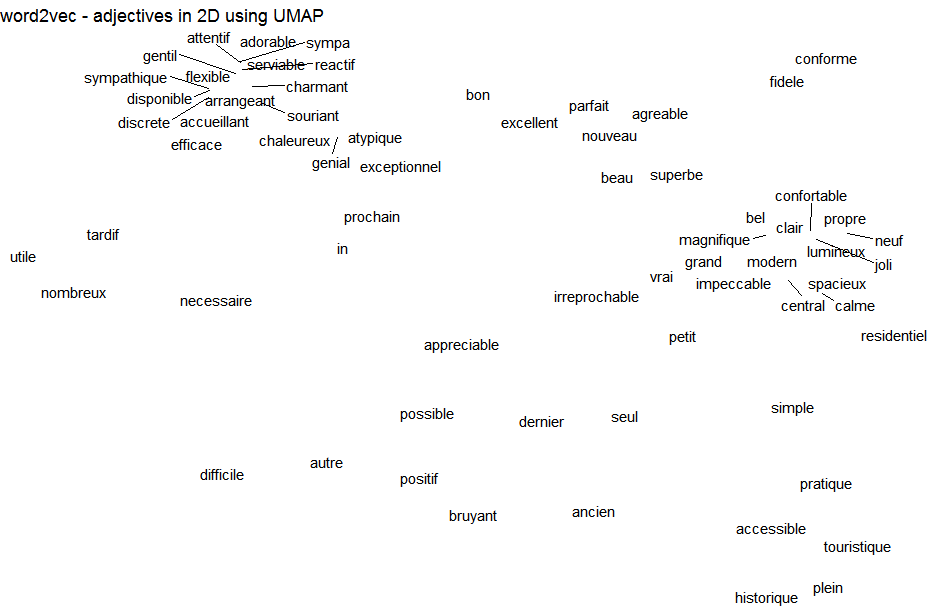
\includegraphics[width=0.6\textwidth]{informatica/word2vec_example}
        \caption{Ejemplo de un \textit{embedding} semántico, computado por el modelo \textit{word2vec} \cite{informatica:word2vec}, de palabras en francés. Imagen extraída de \url{https://cran.r-project.org/web/packages/word2vec/readme/README.html}}
    \end{figure}

    En el caso concreto de \cite{informatica:word2vec}, que propone el conocido modelo \textit{word2vec}, se consigue que el \textit{embedding} tenga cierta \entrecomillado{estructura algebraica}, pudiendo computar, por ejemplo:

    \begin{equation}
        vector("rey") - vector("hombre") + vector("mujer") = vector("reiina")
    \end{equation}
\end{ejemplo}

\begin{ejemplo}
    Veamos ahora un ejemplo mucho más cercano con el problema que queremos resolver. Por ejemplo, el problema de re-identificación (ambiente en el que se proponen las nuevas técnicas de cómputo del \textit{triplet loss} \cite{informatica:principal}).

    En este caso, queremos que las imágenes de una persona en una escena, se transformen a vectores cercanos, como muestra la siguiente representación:

    \begin{figure}[H]
        \centering
        \includegraphics[width=0.6\textwidth]{informatica/embedding_paper_principal}
        \caption{Imagen extraída de \cite{informatica:principal}. Se representa una proporción del \textit{dataset} \textit{Market-1501} tras aplicar el \textit{embedding} aprendido y posteriormente \textit{t-SNE}}
    \end{figure}

    Por ejemplo, un modelo que quiera resolver esta tarea podría aprender a mapear personas con exactamente la misma ropa a puntos cercanos.
\end{ejemplo}

\begin{ejemplo}

    Y para finalizar, consideremos nuestra tarea en concreto. Buscamos que las imágenes de la misma persona, aunque hayan pasado los años, se transformen en vectores cercanos. Y al contrario, que imágenes de dos personas distintas estén lo más lejos posible.

    Esto es especialmente complicado, como ya hemos comentando en \customref{ich:descrp_problema}, porque por ejemplo, nuestro modelo debe ver como más cercanos imágenes de un niño y un adulto con barba (ambos siendo la misma persona) que dos imágenes de dos adultos con barba (siendo distintas personas), como hemos mostrado claramente en \customref{img:messi_distintos_otro_adulto}

\end{ejemplo}

\section{\textit{Triplet Loss}} \label{isec:triplet_loss}

Nuestro objetivo es ahora justificar el uso de \textit{triplet loss} como una función de pérdida que permita a nuestro modelo aprender un \textit{embedding} semántico.

Recordemos que estamos trabajando con funciones de la forma:

\begin{equation}
\begin{split}
    f_{\theta}: X & \to \R^N \\
    x & \mapsto f_{\theta}(x)
\end{split}
\end{equation}

y con una métrica:

\begin{equation}
\begin{split}
    D: X \times X & \to [0, \infty) \\
    x, y & \mapsto D(x, y)
\end{split}
\end{equation}

Para ser más concisos, usaremos la notación $D_{i, j} := D(f_{\theta}(x_i), f_{\theta}(x_j))$.

Como su nombre indica, \textit{triplet loss} trabajará sobre triples. Esto es:

\begin{enumerate}
    \item Una imagen de un individuo concreto, a la que llamaremos \textbf{\textit{anchor}} o ancla
    \item Otra imagen distinta, pero del mismo individuo, a la que llamaremos \textbf{positivo}
    \item Una imagen de un individuo distinto, a la que llamaremos \textbf{negativo}
\end{enumerate}

En este caso, queremos que la distancia entre el \textit{embedding} del ancla y el positivo (que podemos denotar $D_{A, P}$) sea mucho menor que la distancia entre el \textit{embedding} del ancla y el negativo (denotamos $D_{A, N}$). Por tanto, lo que realmente queremos es que:

\begin{equation}
    D_{A, P} \leq D_{A, N}
\end{equation}

o lo que es lo mismo,

\begin{equation}
    D_{A, P} - D_{A, N} \leq 0
\end{equation}

Una forma trivial de hacer que esa ecuación se cumpla, es haciendo que

\begin{equation}
    f(x) = \vec{0}; \dspace \forall x \in X
\end{equation}

con lo que obtendríamos un modelo totalmente inservible. Para evitar eso, introducimos un término $\alpha > 0$ que se conoce como \textbf{margen}, llegando a:

\begin{equation}
    D_{A, P} - D_{A, N} + \alpha \leq 0
\end{equation}

Buscamos que el término de la izquierda sea lo más negativo posible, por lo buscamos minimizar la siguiente función de pérdida:

\begin{equation} \label{ieq:triplet_loss_single_entry}
\begin{split}
    \mathcal{L}_{tri}(\theta; A, P, N) & := max \{D_{A, P} - D_{A, N} + \alpha, 0 \} = \ldots \\
    \ldots &= ReLU(D_{A, P} - D_{A, N} + \alpha)
\end{split}
\end{equation}

Minimizando esta función de pérdida, lo que haremos será atraer elementos de la misma clase entre sí, y alejar elementos de clases distintas. Este proceso se refleja en la siguiente imagen:

\begin{figure}[H]
    \centering
    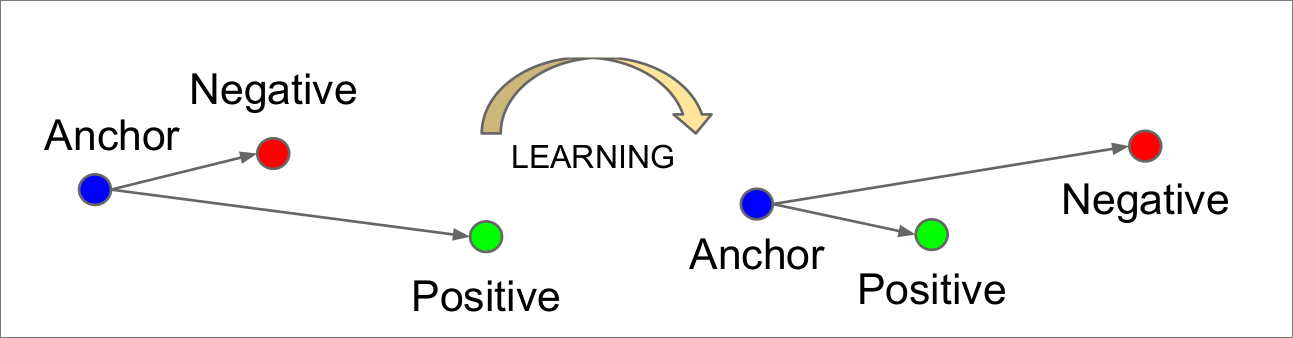
\includegraphics[width=0.8\textwidth]{informatica/triplet_loss_learning}
    \caption{Ejemplo gráfico del proceso de aprendizaje deseado con \textit{triplet loss}. Imagen extraída de \cite{informatica:facenet}}
\end{figure}

Sin embargo, en \eqref{ieq:triplet_loss_single_entry} trabajamos con una sola entrada de tres datos. A diferencia de un \textit{dataset} con datos etiquetados clásico (de la forma \lstinline{(entrada, valor de etiqueta)}), tenemos datos de la forma \lstinline{(imagen, identificador de individuo, edad)}. Esto supone un \textbf{problema} a resolver: cómo generamos \textit{batches} con triples de la forma \lstinline{(ancla, positivo, negativo)} para poder aplicar \eqref{ieq:triplet_loss_single_entry}. Introducimos algunas soluciones propuestas a este problema en \customref{isec:batching}

Por otro lado, este enfoque plantea algunas \textbf{ventajas}. La principal es que, a diferencia de otros enfoques basados en usar funciones de pérdida auxiliares (y que suelen fuerzan que la red solo pueda funcionar comparando pares de imágenes), el cómputo del \textit{embedding} es directo usando esta función de pérdida (\textit{end to end learning}). Optimizamos directamente la propiedad semántica del \textit{embedding} que deseamos obtener. Una vez entrenado el modelo es directo adaptar el modelo a tareas de \textit{clustering}, \textit{retrieval}, verificación, \ldots \cite{informatica:principal}

\section{Generación de \textit{batches}} \label{isec:batching}

Como ya hemos comentado, la tarea que debemos resolver ahora es la de generación de \textit{batches} adecuados para poder emplear \eqref{ieq:triplet_loss_single_entry} como función de pérdida a minimizar.

Por tanto, dado un conjunto de datos de la forma \lstinline{(imagen, identificador, edad)}, debemos obtener un conjunto de datos de la forma \lstinline{(img. ancla, img. positivo, img. negativo)}. Este último conjunto de datos puede ser una lista de triples o conjuntos de \textit{batches}. Como vamos a trabajar con \textit{batches}, podemos simplemente muestrear aleatoriamente y sin remplazo de la lista de triples, repitiendo el muestreo tras cada época completada.

\subsection{Enfoque \textit{offline}} \label{isubs:enfoque_offline_minado_triples}

Este es el enfoque clásico, que se ha venido usando previo a \cite{informatica:facenet}, que introduce un enfoque \textit{online} que luego otros trabajos como \cite{informatica:principal} han ido mejorando.

En este enfoque, el ciclo de aprendizaje se divide en \textbf{varios pasos}.

En primer lugar, se realiza un \textbf{minado \textit{offline}} de los triples. Es decir, se obtiene una primera lista (o conjunto de \textit{batches}) de la forma \lstinline{(img. ancla, img.positivo, img.negativo)}. Una forma de hacer esto sería, por ejemplo, generar los triples de forma aleatoria, generar todos los posibles triples, $\ldots\dspace$ Aunque estas ideas no suelen funcionar en la práctica. Otra forma más efectiva es seleccionar los triples en base de algún estudio estadístico. O usar la red que vamos a optimizar, para identificar aquellos triples en los que tiene más dificultad de distinguir.

En segundo lugar, realizamos el aprendizaje sobre dicho conjunto de triples. En algunos casos, realizamos el entrenamiento completo sobre dicho conjunto inicial. En otros casos, principalmente cuando usamos la red para el minado de triples, pasadas algunas épocas de entrenamiento volvemos a generar otra vez la lista de triples. Así, triples que antes la red no identificaba propiamente, ahora sí que los identifica (\entrecomillado{network snapshots}, \cite{informatica:facenet}) y podemos buscar triples más interesantes.

Una vez computado una lista de triples $(a, p, n) \in \Omega$, la función de pérdida \eqref{ieq:triplet_loss_single_entry} se implementa de forma natural como en cualquier otro ámbito de \textit{batching}:

\begin{equation}
    \mathcal{L}_{tri}^{offline}(\theta; \Omega) := \frac{1}{\#\Omega} \sum_{(a, p, n) \in \Omega} \mathcal{L}_{tri}(\theta; a, p, n)
\end{equation}

\begin{observacion}

Normalmente, en la literatura sobre aprendizaje automático, se ignora el término $\frac{1}{\#\Omega}$ y se supone que siempre estamos dividiendo por el número de sumandos, con lo que nuestra función de error suele escribirse como:

\begin{equation}
    \mathcal{L}_{tri}^{offline}(\theta; \Omega) := \sum_{(a, p, n) \in \Omega} \mathcal{L}_{tri}(\theta; a, p, n)
\end{equation}


\end{observacion}

Este enfoque supone una serie de \textbf{problemas}:

\begin{itemize}
    \item Estamos dividiendo el proceso de aprendizaje en dos etapas, la de minado de triples y la de aprendizaje sobre estos triples. Esto añade complejidad a nuestra \textit{pipeline}
    \item La adecuada elección de triples es fundamental. Si elegimos triples demasiado fáciles, la red no aprenderá nada nuevo, pues es muy fácil distinguir los ejemplos presentados. Sin embargo, si solo mostramos triples complicados, el modelo se centrará en aprender ejemplos extraordinarios y no sabrá distinguir el grueso de ejemplos más sencillos
        \begin{itemize}
            \item Además, generalmente los modelos aprenden rápidamente a distinguir la mayoría de ejemplos en los que las diferencias son relativamente evidentes. Por tanto, en pocas iteraciones la mayoría de triples son demasiado sencillos, lo que agrava mucho este problema
        \end{itemize}
    \item Lo ideal sería disponer de alguna forma de ajustar la complejidad de los triples presentados. Podemos confiar en que al ir re-generando la lista de triples, la complejidad vaya aumentando. Pero el algoritmo de minado debería tener alguna forma de controlar el énfasis que se hace en la búsqueda de combinaciones difíciles, lo que añade aún más complejidad al sistema
    \item El minado supone realizar un proceso de búsqueda, que es \textbf{muy lento} (evaluar de alguna forma todos los posibles triples supondría al menos $O(n^3)$). Lo ideal sería disponer de algún método que se basará en muestrear aleatoriamente de nuestra lista de \lstinline{(imagen, identidad, edad)} (proceso que es muy rápido) y generar rápidamente triples interesantes (esto es lo que hacemos en \customref{isubs:triples_online})
\end{itemize}

\subsection{Enfoque \textit{online}} \label{isubs:triples_online}

La idea común será implementar el siguiente proceso. En primer lugar, realizaremos un muestreo aleatorio sobre los datos de la forma \lstinline{(imagen, identidad, edad)}. Este muestreo es rápido y no supone prácticamente tiempo de cómputo. Usando únicamente los datos de ese muestreo, generaremos triples y computaremos la función de pérdida apoyándonos en \eqref{ieq:triplet_loss_single_entry}. Dicha generación ya sí que supone un tiempo de cómputo considerable. Repetimos este proceso hasta agotar todos las entradas de nuestro \textit{dataset}, completando así una época de entrenamiento.

Ya podemos ver algunas \textbf{ventajas de este método}, incluso antes de haber especificado las dos partes fundamentales (muestreo y selección de triples):

\begin{enumerate}
    \item La ventaja más obvia es que, suponiendo que el tamaño de la muestra es significativamente mucho más pequeño que el tamaño de todo el conjunto de datos, la generación de triples consumirá potencialmente menos tiempo y será más efectiva
        \begin{itemize}
            \item Para afirmar esto rotundamente, tendríamos que realizar un estudio del tiempo del minado \textit{offline} en contraste a la suma de todos los tiempos de minado en cada muestreo
            \item Sin embargo, el tiempo usado es más eficiente, porque en cada paso estamos usando la red actualizada. En el minado \textit{offline} podemos gastar muchísimo tiempo en encontrar triples difíciles que, tras entrenar en pocos ejemplos previos, acaben siendo sencillos, y por tanto, cuando la red vea estos ejemplos, ya sean totalmente inútiles
        \end{itemize}
    \item Se facilita en gran parte el ajuste de la dificultad. Podemos buscar triples realmente difíciles, pero como solo se tiene acceso a una pequeña muestra, estamos controlando la dificultad. Aquí podemos variar el tamaño de las muestras para buscar un punto medio entre ejemplos muy difíciles o ejemplos demasiado sencillos. Y todo esto sin contar con el factor de que vamos a usar la red actualizada para la elección de los triples, como comentaremos más adelante
\end{enumerate}

Desarrollada esta visión de forma general, veamos cómo se implementa cada una de las partes, siguiendo las técnicas introducidas en \cite{informatica:principal}.

\subsection{Muestreo de los datos con \textit{P-K sampling}}

La \textbf{idea principal del muestreo} es lo que definiremos como \textbf{\textit{P-K sampling}}. Como ya hemos comentado en \customref{isubs:triples_online}, nuestra tarea ahora es generar un \textit{batch} de elementos de la forma \lstinline{(imagen, identidad, edad)}. En una segunda etapa (véase \customref{isubs:seleccion_de_triples}), otro algoritmo decide como generar triples a partir de estos datos.

El algoritmo de muestreo \textit{P-K sampling} es muy sencillo. En cada muestreo, seleccionamos aleatoriamente $P$ identidades de individuos (o clases, en un ambiente más general en el que no necesariamente estemos trabajando con imágenes de personas). Por cada una de las identidades, seleccionamos aleatoriamente $K$ imágenes. Por tanto, obtenemos una lista de $P \cdot K$ imágenes, o lo que podemos llamar, un \textbf{\textit{P-K batch}}. Para poder obtener triples interesantes en la siguiente etapa, parece que lo deseable es que ambas selecciones aleatorias (muestreos) sean sin repetición.

El hecho de tener $K$ imágenes por cada uno de los individuos seleccionados es lo que va a permitir al algoritmo de generación de triples obtener rápidamente triples interesantes.

Queda aquí claro los problemas que introduce este muestreo: si queremos muestrear $K$ imágenes de cada individuo sin repetición, cada individuo debe tener asociadas al menos $K$ imágenes. Así que a la hora de trabajar con un \textit{dataset}, siempre deberíamos comprobar la distribución del número de imágenes por individuo, como hemos hecho en \customref{isec:base_datos_usada}.

\subsection{Selección de triples y funciones de pérdida} \label{isubs:seleccion_de_triples}

Una vez que tenemos un \textit{batch} de $P \cdot K$ elementos, deberemos seleccionar triples de ellos. Una vez se especifica cómo se seleccionan los triples, usando \eqref{ieq:triplet_loss_single_entry}, inducimos de forma natural y directa una cierta función de pérdida que actúa sobre estos \textit{P-K batches}.

\begin{observacion}

    Vamos a trabajar con $P \cdot K$ elementos, cada uno correspondiendo a una clase en concreto. Por tanto, indexaremos los elementos de la forma $x_k^p$ donde $p$ marca el identificador del individuo, y $k$ marca a cuál de las $K$ imágenes del individuo $p$ nos estamos refiriendo

\end{observacion}

\subsubsection{\textit{Batch Hard}} \label{isubsubs:batch_hard}

La primera idea es iterar sobre todos los elementos del \textit{P-K batch}, obteniendo así $P \cdot K$ anclas. Por cada ancla, seleccionamos el positivo y negativo \textbf{más complicado dentro de \textit{P-K batch}}. Por tanto, queda claro que \textbf{estamos usando la red para seleccionar triples difíciles} en cada \textit{batch} generado.

Esto introduce la siguiente función de pérdida, a la que llamaremos \textbf{\textit{Batch Hard}}:

\begin{equation}
    \mathcal{L}_{BH}(\theta, \hat{\Omega}) := \comentarencima{\sum_{p = 1}^P \sum_{k = 1}^K}{\text{todas las anclas}} [
        \comentarencima{\max_{k' = 1, \ldots, K} D(f_{\theta}(x_k^p), f_{\theta}(x_{k'}^p))}{\text{positivo más complicado}}
        - \comentarencima{\min_{\substack{p' = 1, \ldots, P \\ p' \neq p \\ k' = 1, \ldots, K}} D(f_{\theta}(x_k^p), f_{\theta}(x_{k'}^{p'}))}{\text{negativo más complicado}}
        + \alpha]_+
\end{equation}

donde $[x]_+ := max \{0, x\} = ReLU(x)$ y $\hat{\Omega}$ se refiere a un \textit{P-K batch}. No olvidemos que no estamos escribiendo la división por el número de sumandos, $P \cdot K$.

Estamos generando \textbf{triples moderados}, porque estamos buscando los triples más difíciles, pero dentro de un \textit{batch} relativamente pequeño comparado a el total del conjunto de datos. Por tanto, estamos ajustando la dificultad de los triples cómodamente, resolviendo el problema que comentábamos en \customref{isubs:enfoque_offline_minado_triples}. Aumentando el valor de $P, K$, aumentamos el espacio de búsqueda, y por tanto podremos encontrar triples mucho más difíciles. Sin embargo, hay que tener siempre en cuenta el coste en tiempo de cómputo.

Queda claro que, gracias al proceso de \textit{P-K sampling}, ahora es factible realizar una búsqueda de triples interesantes en profundidad, basándonos en el estado más actualizado de la red para calcular la dificultad de los triples. Esta búsqueda extensiva no habría sido posible si la planteásemos sobre todo el conjunto de datos.

\subsubsection{\textit{Batch All}} \label{isubsubs:batch_all}

Motivados por lo comentado en \customref{isubsubs:batch_hard}, podemos plantearnos usar todas los posibles triples dentro de un \textit{P-K batch} como un enfoque que ahora cobra más sentido (ya hemos comentado en \customref{isubs:enfoque_offline_minado_triples} que realizar esto sobre todo el conjunto de datos no parece una buena idea).

Realizar esto introduce la función de pérdida que llamaremos \textbf{\textit{Batch All}}:

\begin{equation} \label{ieq:batch_all}
    \mathcal{L}_{BA}(\theta; \hat{\Omega}) :=
    \comentarencima{\sum_{p = 1}^{P} \sum_{k = 1}^K}{\text{todas anclas}}
    \comentardebajo{\sum_{\substack{k' = 1 \\ k' \neq k}}^{K}}{\text{todas pos.}}
    \comentarencima{\sum_{\substack{p' = 1 \\ p' \neq p}}^P \sum_{n = 1}^K}{\text{todas neg.}} \dspace[
        D(f_{\theta}(x_k^p),f_{\theta}(x_{k'}^p)) - D(f_{\theta}(x_k^p),f_{\theta}(x_{n}^{p'})) + \alpha
    ]_+
\end{equation}

Está claro que, por el número de sumandos, esta aproximación es viable gracias a que nuestro \textit{P-K sampling} reduce mucho el número de elementos sobre los que operamos. Dicho número de sumandos viene dado por:

\begin{equation}
    P \cdot K \cdot (K - 1) \cdot (P - 1) \cdot K = P^2 - P + K^3 - K^2 \approx P^2 + K^3
\end{equation}

Esta aproximación sería completamente inviable sobre un número muy elevado de elementos. Pensemos, por ejemplo, en las 163446 imágenes de \textit{CACD}.

\subsubsection{Mejoras introducidas a partir de la experimentación}

En \cite{informatica:principal}, a raíz de observar los resultados de la experimentación, señalan algunos puntos débiles en las dos funciones de pérdida que introducen a partir del \textit{P-K sampling}.

Principalmente, en \customref{isubsubs:batch_all}, podemos ver un posible fallo en la función de pérdida \eqref{ieq:batch_all}. Si se da el caso de que la mayoría de triples generados son fáciles (hecho muy probable al estar generando todas las combinaciones de triples), los escasos triples que realmente son difíciles se desvanecerán. Esto porque la mayoría de términos serán cero (al estar aplicando $[x]_+$). Y los pocos términos que no son cero, se dividen por el número total de elementos, que ya hemos visto que es elevado.

Por tanto, una mejora sencilla a esta función de pérdida es dividir únicamente por el número de sumandos no nulos. Esta mejora la podemos aplicar también a \textit{batch hard}, obteniendo dos nuevas funciones de pérdida, a las que llamaremos $\mathcal{L}_{BA \neq 0}$ y $\mathcal{L}_{BH \neq 0}$.

\subsubsection{Algunas observaciones y conclusiones}

En primer lugar, cabe destacar que, como señalan \cite{informatica:principal}, las dos nuevas funciones de pérdida introducidas equivalen al planteamiento clásico de \textit{triplet loss} si entrenásemos indefinidamente.

El desarrollo que hemos realizado justifica las siguientes \textbf{ventajas} de los nuevos métodos:

\begin{itemize}
    \item El uso del \textit{P-K sampling} y las dos nuevas funciones de pérdida (con las variantes técnicas) permiten realizar el aprendizaje de forma usual, sin añadir un paso adicional en el bucle de aprendizaje, evitando así la gran complejidad añadida del minado \textit{offline}
    \item Además, conseguimos un manejo preciso de la dificultad de los triples obtenidos. Controlando el valor de $\{P, K\}$, controlamos el espacio de búsqueda y, en definitiva, la dificultad. Todo esto de forma cómoda y sin introducir apenas complejidad en nuestro \textit{pipeline}
    \item Aunque no lo hemos comprobado, pensamos que esto acelera los tiempos de cómputo, al estar realizando el minado de triples sobre \textit{batches} de tamaño considerablemente reducidos
    \item Y aunque no mejorásemos el tiempo de computo, lo que sí sabemos que mejoramos es la eficacia del minado de triples. El minado de triples usa una red mucho más actualizada, para generar una lista mucho más pequeña que probablemente no se degrade tanto como la generada por un minado \textit{offline} sobre todo el conjunto de datos, mucho más grande
    \item Es más, estamos controlando el efecto de los triples demasiado sencillos, que no tendremos en cuenta a la hora de dividir los sumandos en la función de pérdida
\end{itemize}

A pesar de esto, a raíz de trabajar con estas nuevas técnicas, identificamos los siguientes \textbf{inconvenientes}:

\begin{itemize}
    \item Introducimos dos hiperparámetros, $\{P, K\}$, que deberemos ajustar correctamente, pues tienen un enorme impacto en los resultados del proceso de entrenamiento. Por tanto, se hace fundamental tener un proceso de \textit{hyperparameter tuning} robusto, como introducimos en \customref{isec:hp_tuning}
    \item Tenemos que tener mucho cuidado con valores elevados de $\{P, K\}$, por dos motivos. El primero, y como ya hemos comentado, valores altos implicarán que los tiempos de cómputo para la generación de triples crecerán rápidamente. El segundo es que el tamaño de los \textit{batches} crecerán considerablemente, llegando a colapsar la memoria disponible de la \textit{GPU}
    \item Hemos comprobado en la práctica que es realmente fácil colapsar la memoria \textit{GPU}, usando modelos profundos como \textit{ResNet50} con valores de $P \cdot K > 200$. Esto supone que, aunque no estuviéramos limitados por el tiempo de cómputo, el colapso de la memoria limita el conjunto de valores que $\{P, K\}$ puede tomar, restringiendo fundamentalmente la experimentación que podemos realizar con estos valores
    \item Si queremos usar valores altos de $K$, nuestro \textit{dataset} lo debe permitir, teniendo una buena distribución de imágenes por individuo (por esto, hemos realizado este estudio en \customref{isec:base_datos_usada} para nuestras bases de datos). Se pueden explorar técnicas como el aumentado de datos para aumentar el número de imágenes por individuo, pero solo serán efectivas si dicha distribución es buena para empezar
    \item Tanto por el formato de los datos con los que hemos trabajado, como por el cambio fundamental realizado en el \textit{sampling} de los datos, hemos tenido que realizar un \textbf{esfuerzo considerable de implementación}, al no poder basarnos en la mayor parte de los casos en código implementado por alguna biblioteca de aprendizaje automático. Esto se ve reflejado en \customref{ich:implementacion}
\end{itemize}

\section{Función de distancia}


\section{Métricas}

\todo{Hablar de rank@k, distancias intracluster, intercluster, silhouette, ...}

\section{Hablar de la tarea de retrieval?}


% -------------------------------------------------------------------
% BACKMATTER
% -------------------------------------------------------------------

\backmatter % Desactiva la numeración de los capítulos
\pdfbookmark[-1]{Referencias e Índices}{BM-Referencias}

% BIBLIOGRAFÍA
%-------------------------------------------------------------------

\bibliographystyle{alpha}
\begin{small} % Normalmente la bibliografía se imprime en un tamaño de letra más pequeño.
\bibliography{references.bib}
\end{small}

\end{document}
